\newpage
\section{LECTURE 11}

\subsection{Agenda}
\begin{itemize}
    \item Dealing with Attitude (Rotation matrice + quaternion)
    \item Optimization with Quaternions
\end{itemize}

\subsection{Attitude}

\begin{figure}
    \centering
    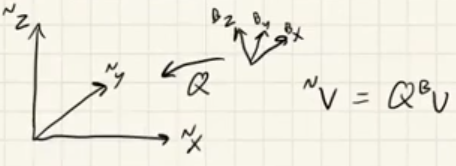
\includegraphics[width=0.4\linewidth]{L11_Images/F1.PNG}
    \caption{Attitude}
    \label{fig:l11f1}
\end{figure}

\begin{itemize}
    \item Many robotic systems undergo large rotations.(quadrotors, airplanes, spacecraft, underwater vehices, legged robots)
    \item Naive angle-based parameterizations (Euler angles) have singularities that cause failures and/pr require hacks.
    \item Rotation matrices and quaternion are singularity free but optimizing over them requires some extra tricks.
    \item What is Attitude?
    \begin{itemize}
        \item Rotation from body frame to world frame
    \end{itemize}
    \item 3DOF, but there is no globally nonsingularity 3-parameter attitude representation.
    \item Rotation/"Direction-Cosine" Matrix
    \begin{align}
        \begin{bmatrix}
            ^N x_1 \\ ^N x_2 \\ ^N x_3
        \end{bmatrix} & = 
        \begin{bmatrix}
            ^b n_1^T \\ --- \\ ^b n_2^T \\ --- \\ ^b n_3^T \\ 
        \end{bmatrix}
        \begin{bmatrix}
            ^B x_1 \\ ^B x_2 \\ ^B x_3
        \end{bmatrix} = 
        \begin{bmatrix}
            ^N b_1 & | & ^N b_2 & | & ^N b_3 
        \end{bmatrix}
        \begin{bmatrix}
            ^B x_1 \\ ^B x_2 \\ ^B x_3
        \end{bmatrix} \\
        \Rightarrow Q^T Q & = I \Rightarrow Q^{-1} = Q^T \Rightarrow \text{"orthogonal"} \\
        \Rightarrow det(Q) & = 1 \\
        Q & \in SO(3) \text{"Special orthogonal group in 3D"}
    \end{align}
\end{itemize}

\subsection{Kinematics (how do I integrate a gyro)}

\begin{figure}
    \centering
    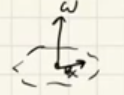
\includegraphics[width=0.2\linewidth]{L11_Images/F2.PNG}
    \caption{Gyro}
    \label{fig:l11f2}
\end{figure}

\begin{align}
    ^N x = Q(t) ^B x, ^N \dot x = ^N \omega \times ^N x = Q(^B \omega \times ^B x)
\end{align}
\begin{itemize}
    \item Apply chain rule:
    \begin{align}
        ^N x & = Q ^B x \Rightarrow ^N \dot x = \dot Q ^B x + Q ^B \dot x = \dot Q ^B x  \\
        \Rightarrow & \dot Q ^B x = Q(^B \omega \times ^B x) \\
        \omega \times x & = 
        \begin{bmatrix}
            0 & -\omega_3 & \omega_2 \\
            \omega_3 & 0 & -\omega_1 \\
            -\omega_2 & \omega_1 & 0 \\
        \end{bmatrix}
        \begin{bmatrix}
            x_1 \\ x_2 \\ x_3
        \end{bmatrix} = \hat \omega x\\
        \Rightarrow & \dot Q ^B x = Q \hat \omega ^B x \Rightarrow \dot Q = Q \hat w
    \end{align}
    \item We could do dynamics with rotation metrices in our state, but has a lot of redundancy.
    \item Quaternion are more compact / efficient.
    \item Define axis of rotation (unit vector) a.
    \item Define angle of rotation (scalar, radians) $\theta$
    \begin{align}
        \phi & = a \theta \\
        \Vert \phi \Vert & = \theta, \frac{\phi}{\Vert \phi \Vert} = a, \phi \in \mathbb{R}^3 \text{"axis-angle" vector} 
    \end{align}

    \item For constant $\omega$ (or short h)) can think of $\phi$ as integral of $\omega$:
    \begin{align}
        \phi \approx \int_0^h \omega dt \text{(not true in general)}
    \end{align}
    \item In term of axis-angle, we can define quaternion:
    \begin{align}
        q = \begin{bmatrix}
            \cos(\frac{\theta}{2}) \\ a \sin (\frac{\theta}{2})
        \end{bmatrix} \\
    \end{align}
    \begin{itemize}
        \item $q^T q = 1 \Rightarrow $ Valid rotations correspond to "unit quaternions", Easy to normalize.
        \item q and -q correspond to the same rotation (add $2 \pi$ to $\theta$), called "double cover".
        \item Opperations on quaternion are analogous to rotation matrices.
    \end{itemize}
    \item Quaernion Multiplication:
    \begin{align}
        \begin{split}
            q_1 * q_2 & = 
            \begin{bmatrix}
                s_1 \\ v_1
            \end{bmatrix} + 
            \begin{bmatrix}
                s_2 \\ v_2
            \end{bmatrix} =
            \begin{bmatrix}
                s_1 s_2 - v_1^T v_2 \\ s_1 v_2 + s_2 v_1 + v_1 \times v_2
            \end{bmatrix} \\
            & = \begin{bmatrix}
                s_1 & -v_1^T \\
                v_1 & s_1I + \hat v_1
            \end{bmatrix}
            \begin{bmatrix}
                s_2 \\ v_2
            \end{bmatrix} 
            = L(q_1)
            \begin{bmatrix}
                s_2 \\ v_2
            \end{bmatrix} \\
            & = \begin{bmatrix}
                s_2 & -v_2^T \\
                v_2 & s_2I - \hat v_2
            \end{bmatrix}
            \begin{bmatrix}
                s_1 \\ v_1
            \end{bmatrix} 
            = R(q_2)
            \begin{bmatrix}
                s_1 \\ v_1
            \end{bmatrix} 
        \end{split}
    \end{align}
    \item Quaternion Identity:
    \begin{align}
        q = 0 \Rightarrow
        \begin{bmatrix}
            1 \\ 0 \\ 0 \\ 0
        \end{bmatrix}
    \end{align}
    \item Quaternion Conjugate
    \begin{align}
        q^* = \begin{bmatrix}
            s \\ -v
        \end{bmatrix} =
        \begin{bmatrix}
            1 & 0 \\
            0 & -I
        \end{bmatrix}
        \begin{bmatrix}
            s \\ v
        \end{bmatrix}
    \end{align}
    \item Rotate a vector:
    \begin{align}
        H & = \begin{bmatrix}
            0 \\ I
        \end{bmatrix} \\
        Hx & = \begin{bmatrix}
            0 \\ ^w x
        \end{bmatrix} = q * \begin{bmatrix}
            0 \\ ^B x
        \end{bmatrix} * q^* = L(q) R^T(q) ^B x = R^T(q) L(q) ^B x \\
        Q(q) & = L(q) R^T(q) = R^T(q) L(q)
    \end{align}
    \item Quaternion Kinematics:
    \begin{align}
        \dot q & = \frac{1}{2} q * \begin{bmatrix}
            0 \\ \omega
        \end{bmatrix} = \frac{1}{2} L(q) H \omega \\
        & L(q) H \in \mathbb{R}^{4 \times 3}
    \end{align}
    \item Now we can simulate dynamics with quaternions.
\end{itemize}

\subsubsection{Geometry of Quaternions:}

$q$ lives on a sphere in $\mathbb{R}^4$ \\
$\dot q$ lives in the tangent plane to the sphere at q. \\

\begin{figure}
    \centering
    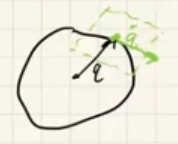
\includegraphics[width=0.2\linewidth]{L11_Images/F3.PNG}
    \caption{Geometry of Quaternions}
    \label{fig:l11f3}
\end{figure}

\begin{figure}
    \centering
    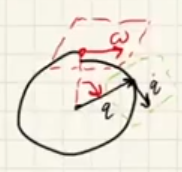
\includegraphics[width=0.2\linewidth]{L11_Images/F4.PNG}
    \caption{Kinematics of Quaternion}
    \label{fig:l11f4}
\end{figure}


\begin{itemize}
    \item Kinematics:
    \begin{align}
        \dot q \in \mathbb{R}^4, \omega \in \mathbb{R}^3, \dot q = \frac{1}{2} q *
        \begin{bmatrix}
            0 \\ \omega
        \end{bmatrix} = \frac{1}{2} L(q) H \omega
    \end{align}
    \begin{itemize}
        \item $\omega$ is always written down in the tangent plane at the identity, then kinematics rotate to the tangent plane centered on q.
    \end{itemize}
    \item Analogy with unit complex number in 2D:
    \begin{align}
        v & = \cos(\theta) + i \sin(\theta) = 
        \begin{bmatrix}
            \cos(\theta) \\ \sin(\theta)
        \end{bmatrix} \\
        \dot v & = \frac{\partial v }{\partial \theta} \dot \theta = 
        \begin{bmatrix}
            - \sin(\theta) \\ \cos(\theta) 
        \end{bmatrix} \dot \theta =
        \begin{bmatrix}
            \cos(\theta) & -\sin(\theta) \\
            \sin(\theta) & \cos(\theta)
        \end{bmatrix}
        \begin{bmatrix}
            0 \\ \dot \theta
        \end{bmatrix}
    \end{align}
    \begin{itemize}
        \item Kinematics rotates $\dot \theta$ from tangent plane at $\theta = 0$ to tangent plane at v.
    \end{itemize} 
\end{itemize}

\begin{figure}
    \centering
    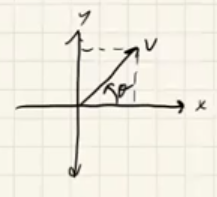
\includegraphics[width=0.2\linewidth]{L11_Images/F5.PNG}
    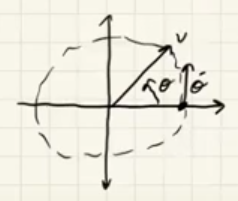
\includegraphics[width=0.2\linewidth]{L11_Images/F6.PNG}
    \caption{2D kinematics rotation}
    \label{fig:l11f5}
\end{figure}

\subsubsection{Differentiating Quaternions:}
\begin{itemize}
    \item Two key facts
    \begin{itemize}
        \item Derivatives are really 3D "tangent vectors"
        \item Rotations compose by multiplication, not addition.
    \end{itemize}
    \item Infinitesimal Rotation
    \begin{align}
        \delta q = \begin{bmatrix}
            \cos(\frac{\theta}{2}) \\ a \sin(\frac{\theta}{2})
        \end{bmatrix} \approx
        \begin{bmatrix}
            1 \\ \frac{1}{2} a \theta
        \end{bmatrix} \approx
        \begin{bmatrix}
            1 \\ \frac{1}{2} \phi
        \end{bmatrix} = 
        \begin{bmatrix}
            1 \\ 0
        \end{bmatrix} + \frac{1}{2}
        \begin{bmatrix}
            0 \\ \phi
        \end{bmatrix} = 
        \begin{bmatrix}
            1 \\ 0
        \end{bmatrix} + \frac{1}{2} H \phi
    \end{align}
    \item Compose with q:
    \begin{align}
        q' & = q * \delta q = L(q) (
            \begin{bmatrix}
                1 \\ 0
            \end{bmatrix} + \frac{1}{2} H \phi
        ) = q + \frac{1}{2} L(q) H \phi \\
        G(q) & = \frac{1}{2} L(q) H \in \mathbb{R}^{4 \times 3} \text{"Attitude Jacobian"}
    \end{align}
    \item Note: We can use any 3-parameter rotation representation for $\phi$. They all linearize the same (up to a constant factor):
    \begin{align}
        \begin{split}
            q & = \begin{bmatrix}
                \cos(\frac{\Vert \phi \Vert}{2}) \\ \frac{\phi}{\Vert \phi \Vert} \sin(\frac{\Vert \phi \Vert}{2})
            \end{bmatrix} \text{axis-angle} \\
            & \approx 
            \begin{bmatrix}
                \sqrt[]{1 - \phi^T \phi} \\ \phi
            \end{bmatrix} \text{vector part of quaternion} \\
            & \approx \sqrt[]{1 + \phi^T \phi}
            \begin{bmatrix}
                1 \\ \phi
            \end{bmatrix} \text{Gibbs/Rodrigues vector}
        \end{split} 
    \end{align}
    \item We'll use the vector part of q in class.
    \item This lets us differentiate w.r.t. quaternions by inserting G(q) in the right places.
    \begin{align}
        f(q) &: \mathbb{H} \to \mathbb{R} \text{ (gardient of a scalar-valued function)} \\
        \mathbb{H} & \text{(quaternion, "Hamilton")} \\
        \nabla f &= \frac{\partial f}{\partial q} \frac{\partial q}{\partial \phi} = \frac{\partial f}{\partial q} G(q) \\
        f(q) &: \mathbb{H} \to \mathbb{H} \text{ (Jacobian of a quaternion-valued function)} \\
        \phi' & = \nabla f \phi (q' = f(q))\\
        \nabla f & = [G^T(f(q)) \frac{\partial f}{\partial q} G(q) ] \in \mathbb{R}^{4 \times 3}
    \end{align}
    \item explaination:
    \begin{align}
        q' &= f(q) \Rightarrow q' \delta q' = f(q \delta q) \\
        q' &* \begin{bmatrix}
            \sqrt[]{1- \phi^T \phi} \\ \phi'
        \end{bmatrix} = 
        f(q * \begin{bmatrix}
            \sqrt[]{1- \phi^T \phi} \\ \phi
        \end{bmatrix}) \\
        \Rightarrow & \frac{\partial \phi'}{\partial \phi} = G^T(f(q)) \frac{\partial f}{\partial q} G(q)
    \end{align}
    \item Hessian of $f(q): \mathbb{H} \to \mathbb{R}$
    \begin{align}
        \nabla^2 f(q) = G^T(q) \frac{\partial^2 f}{\partial q^2} G(q) + I_3 (\frac{\partial f}{\partial q} q)
    \end{align}
    \item Now we can do Newton's method and DDP and SQP with quaternions.
\end{itemize}

\subsection{Example: Pose Estimation}

\begin{itemize}
    \item Given a bunch of vectors to known features in the environment, determine the robot's attitude.
    \item Called "Wahba's Problem"
    \begin{align}
        \min_q J(q) = \sum_{k=1}^m \Vert ^N x_k - Q(q) ^Bx_k \Vert_2^2 = \Vert r(q) \Vert_2^2
    \end{align}
    \item $^N x_k$ and $^B x)k$ are unit vectors ("directions")
    \begin{align}
        r(q) & = 
        \begin{bmatrix}
            ^N x_1 - Q ^B x_1 \\
            ^N x_2 - Q ^B x_2 \\
            ...\\
            ^N x_m - Q ^B x_m 
        \end{bmatrix} \in \mathbb{R}^{3m \times 1} \\
        \Rightarrow 
        \nabla r(q) & =  \frac{\partial r}{\partial q} G(q) \in \mathbb{R}^{3m \times 3}
    \end{align}
\end{itemize}

\subsubsection{Background: Gauss-Newton for Least-Squares}
\begin{align}
    \min_x J(x) & = \frac{1}{2} \Vert r(x) \Vert_2^2 = \frac{1}{2}r(x)^T r(x) \\
    \frac{\partial J}{\partial x} & = r(x)^T \frac{\partial r}{\partial x} \\ 
    \frac{\partial^2 J}{\partial x^2} & = (\frac{\partial r}{\partial x})^T (\frac{\partial r}{\partial x}) + (I \otimes r(x)^T \frac{\partial^2 vec(r)}{\partial x^2} \\
    \Rightarrow (\frac{\partial^2 J}{\partial x^2})^{-1} \nabla J & \approx [(\frac{\partial r}{\partial x})^T (\frac{\partial r}{\partial x})]^{-1} \frac{\partial r}{\partial x}^T r(x)
\end{align}

\subsubsection{Gauss-Newton Method for Wahba's Problem}

\\
\noindent
\begin{algorithm}
	\caption{Gauss-Newton for Wahba's Problem}
	\label{alg:ForwardRollout}
	\begin{algorithmic}[1]	
        \State $q \gets q_0$
	    \While {$\Vert r(q) \Vert > tol} 
            \State $\nabla r(q) = \frac{\partial r}{\partial q} G(q)$ 
            \State $\phi = -[(\nabla r^T \nabla r)^{-1} \nabla r^T] r(q)$
            \State $q \gets q * \begin{bmatrix}
                \sqrt[]{1 - \phi^T \phi} \\ \phi
            \end{bmatrix} $ \Comment{multiplication update}
            \State (In general, do a line search)
        \Endwhile
	\end{algorithmic}
\end{algorithm}
\\

Remember to check out the lecture video for the example code.
